% vim: set tw=78 sts=2 sw=2 ts=8 aw et ai:
\documentclass[paper=a4, fontsize=11pt]{scrartcl}
\usepackage[T1]{fontenc}
\usepackage{fourier}

\usepackage[english]{babel}															% English language/hyphenation
\usepackage[protrusion=true,expansion=true]{microtype}	
\usepackage{amsmath,amsfonts,amsthm} % Math packages
\usepackage[pdftex]{graphicx}	
\usepackage{url}


%%% Custom sectioning
\usepackage{sectsty}
\allsectionsfont{\centering \normalfont\scshape}


%%% Custom headers/footers (fancyhdr package)
\usepackage{fancyhdr}
\pagestyle{fancyplain}
\fancyhead{}											% No page header
\fancyfoot[L]{}											% Empty 
\fancyfoot[C]{}											% Empty
\fancyfoot[R]{\thepage}									% Pagenumbering
\renewcommand{\headrulewidth}{0pt}			% Remove header underlines
\renewcommand{\footrulewidth}{0pt}				% Remove footer underlines
\setlength{\headheight}{13.6pt}


%%% Equation and float numbering
\numberwithin{equation}{section}		% Equationnumbering: section.eq#
\numberwithin{figure}{section}			% Figurenumbering: section.fig#
\numberwithin{table}{section}				% Tablenumbering: section.tab#


%%% Maketitle metadata
\newcommand{\horrule}[1]{\rule{\linewidth}{#1}} 	% Horizontal rule

\title{
		%\vspace{-1in} 	
		\usefont{OT1}{bch}{b}{n}
		\normalfont \normalsize \textsc{Facultatea de Automatica si Calculatoare} \\ [25pt]
		\horrule{0.5pt} \\[0.4cm]
		\huge Referat Laboratorul 4 - Tehnologii avansate utilizate in sistemele cu procesoare
        grafice \\
		\horrule{2pt} \\[0.5cm]
}
\author{
		\normalfont 								\normalsize
        Deaconu Ioan\\[-3pt]		\normalsize
        \today
}
\date{}

\begin{document}
 
\maketitle

\section{Introducere}
\label{sec:introducere}
Intel, pe langa AMD, este unul din liderii mondiali ai industriei de microprocesoare. Acest lucru
este datorat in mare parte arhitecturii Core i7, arhitectura revolutionara lansata in noiembrie
2008.

Desi de atunci Intel a ajuns la a 5-ea iteratie a arhitecturii, sub nume de cod Broadwell, functionarea
 ei este identica cu cea a arhiecturii Nehalem, prima iteratie a lui Core i7.

Din aceast motiv, aceasta lucrare va prezenta imbunatatirile aduse acestei arhitecturi, imbunatari care
chiar si dupa 7 ani de la introducere lor sunt inca folosite si de actualitate.



\section{Notiuni Teoretice Aferente}
\label{sec:notiuniteoretice}
Pentru a putea executa o instructiune, aceasta trebuie citita, decodata, executa si scrise datele
inapoi in memorie. Acesti pasi au fost impartiti in componente simple, pentru a putea face
procesorul mai modular. Acesti pasi, in arhitectura clasica RISC sunt:
\begin{itemize}

\item Instruction Fetch.
\item Instruction Decode and register Fetch.
\item Execute.
\item Memory access.
\item Write Back.

\end{itemize}

\subsection{Scalar - Pipeline}

Din cauza faptului ca doar un singur modul este activ iar celelalte nu fac nimic, incepand cu ani 70
s-a folosit principul de pipeline. Astfel, pentru a se eficientiza utilizarea procesorului, mai
multe instructiuni vor fi executa in acelasi timp, dar decalate cu un pas, pentru a putea folosi
modulele mai eficient.

De exemplu, in cazul a 5 instructiuni, daca consideram ca toate stagiile dureaza 1 unitate de timp,
atunci fara pipeline ar dura 25 de unitati de timp executia totala a instructiunilor. Folosind
pipeline, timpul total de executie al celor 5 instructiuni ar fi de doar 9 unitati de timp
\cite{johnson1991superscalar}.

\begin{figure*}[ht] \centering
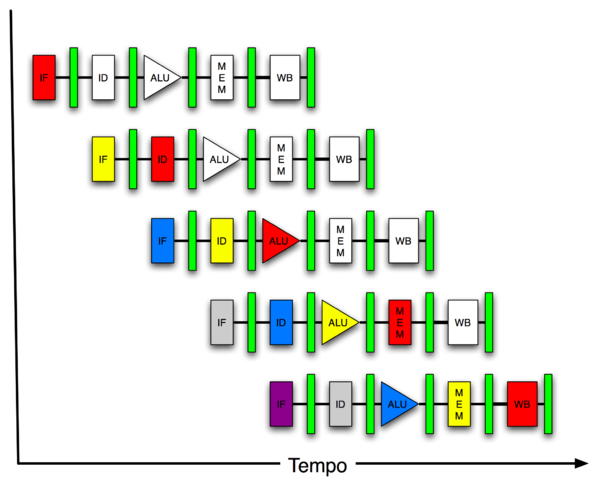
\includegraphics[width=0.9\textwidth]{img/pipeline.png}
\caption{Exemplu de executie a instructiunilor folosind pipeline.} \end{figure*}

\subsection{Scalar Avansat}

Cu timpul, odata ce unitatile interne ale procesorului au devenit din ce in ce mai puternice,
pipelineul a devenit din ce in ce mai lung, ajungand in Pentium 4 la un numar de 31 de stagii de
pipeline. Desi teoretic un pipe lung permite o granularitate mai buna, dezavantajul major il
constituie branchurile, deoarece tot pipeline-ul trebuie golit si incarcat cu instructiuni noi.
Deasemenea un pipeline mai lung inseamna o durata mai mare de executie a unei instructiuni, dar
permite atingerea unor frecvente mai mari. 

Deoarece exista unitati care pot fi nefolosite, spre exemplu floating point unit nu este
folosita cand se executa o instructiune de load sau store, dezvoltatorii de procesoare au decis sa
execute mai multe instructiuni in paralel. Astfel pipelineul pe langa numarul de stagii care le are
a fost marit si in latime. Mai exact, in loc de executia unei singuri instructiuni, se
citesc simultan mai multe instructiuni si se executa simultan. Acest mod de abordare ar permite ,
de exemplu ca in acelasi timp in care se executa adunarea a 2 registre sa se poata compara alte
registre\cite{jouppi1989available}.

\begin{figure*}[ht] \centering
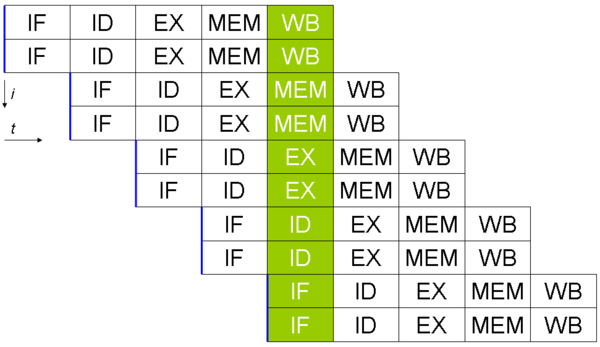
\includegraphics[width=0.9\textwidth]{img/superscalar.png}
\caption{Exemplu de executie a mai multor instructiunilor folosind super scalar.} \end{figure*}




\section{Implementare}
\label{sec:implementare}
\subsection{Accesul nealiniat la memoria cache}

Cea mai mare instructiune de tip SSE are 16 bytes, sau 128 de biti. Pentru fiecare operatie de tip
store/load exista 2 versiuni: prima versiune care are operatorii aliniati la 16 bytes, si cea de-a
doua versiunea care nu are operatorii aliniati.

Compilatoarele folosesc operatiile nealinitate daca nu pot garanta accesul aliniat
la memorie. Toate procesoarele de generatie anterioara, Core 2, aveau o scadere drastica a
performantei in momentul folosirii instructiunilor nealiniate fata de cele aliniate.

Problema este ca majoritatea compilatoarelor nu pot garanta aliniarea datelor in memorie si astfel
se folosesc foarte multe instructiunii nealiniate. Incepand cu arhitectura Nehalem, nu mai exista
scadere de performanta datorata folosirii instructiunilor pe date nealiniate. Astfel compilatoarele
nu vor mai fi nevoie sa alinizeze datele in memorie de teama scaderii vitezei de executie
\cite{thomadakis2011architecture}.

\subsection{Hyper-Threading}

Acesul nealiniat la memorie a fost necesar deoarece in aceasi arhitectura exista simultaneous
multithreading.

In mod normal, un procesorul nu are folosite toate modulele componente in acelasi timp, astfel ca
simultaneous multithreading foloseste aceasta ideea prin simularea a 2 nuclee virtuale folosind un
singur nucleu. Pentru acest lucru, a fost necesara marirea numarului de registrii de load de la 32
la 48 si numarul de registrii de store de la 20 la 32.

\begin{figure*}[ht] \centering
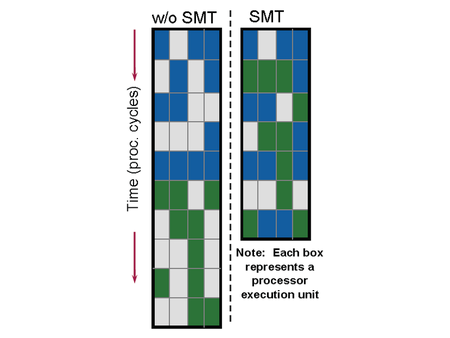
\includegraphics[width=0.6\textwidth]{img/smp.png}
\caption{Diferenta intre cu si fara Hyper-Threading } \end{figure*}

Exista arhitecturi in care se un nucleu fizic poate simula 4 nuclee virtuale, dar in cazul lui Core
i7, Intel a decis sa foloeasca doar 2 nuclee virtuale pentru fiecare nucleu fizic. Astfel in cazu
in care pe un nucleuz s-ar executa operatii cu intregi, unitatea in virgula mobile, ar putea fi
utilizata de un alt thread care ar dori sa foloseasca operatii cu numere reale \cite{semin2009inside}.


\subsection{Controlul Avansat al Consumului}

Intel Core i7 are 4 stari principale ale consumului\cite{power}.

\begin{itemize}
\item P-State - starea de performanta maxima a microprocesorului
\item T-State - starea de sleep in care microprocesorul are frecventa redusa
\item C-State - starea in care procesorul este in sleep
\item S-State - starea de sleep ale sistemului
\end{itemize}

\begin{figure*}[ht] \centering
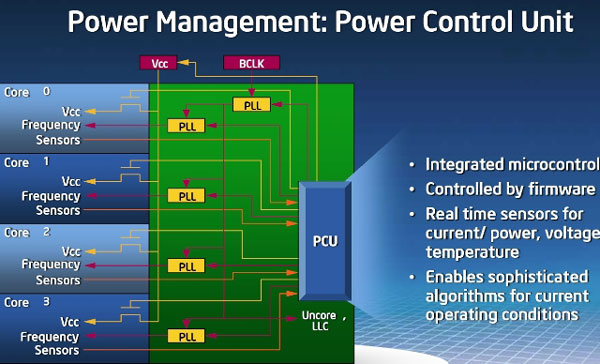
\includegraphics[width=0.6\textwidth]{img/pcu.jpg}
\caption{Unitatea de control a puterii } \end{figure*}

\subsection{Modul Turbo Boost}
Datorita existentei unui control dedicat al puterii, nucleele pot rula la frecvente independente.
In cazul in care doar 2 nuclee din 4 sunt folosite, atunci cele 2 nuclee vor putea rula la o
frecventa mai mare decat cea de baza , deoarece vor folosi puterea salvata prin inchiderea
celorlate 2 nuclee. De exemplu, daca frecventa de baza a unui procesor cu 4 nuclee este de 2,66 ghz
atunci daca maxim 2 nuclee sunt folosite, acestea vor puteea rula la o frecventa maxima de 3 ghz.

\cite{gelsinger2008intel}.

\begin{figure*}[ht] \centering
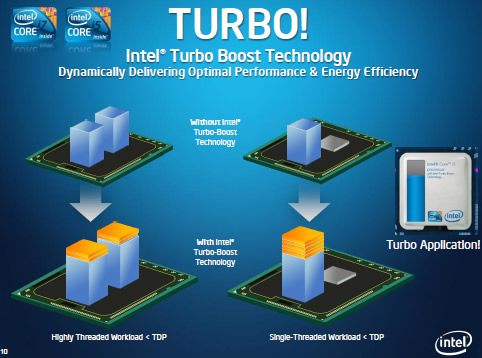
\includegraphics[width=0.6\textwidth]{img/turbo.jpg}
\caption{Exemplu de Turbo Boost } \end{figure*}




\section{Simulare} 
\label{sec:simulare}

Simultaneous Multi-Threading reprezinta cea mai avansata forma de arhitectura superscalara. Pentru
a verifica avantajale ei, am inclus un benchmark din articolul \cite{tuck2003initial}.

In acel test, se verifica cat de mult poate mari viteza de executie folosind SMT. Dupa cum se
observa pe rezultate, speedup-ul mediu este de aproximativ 1.2. Exista cazuri in care speedup-ul
este sub 1, dar sunt rare. Acest test arata ca prin dublarea registriilor si folosirea arhitecturii
superscalare deja existentente, o marirea de aproximativ 5\% a unui nucleu rezulta intr-o crestere
a performantei de pana la 40\%.

\begin{figure*}[ht] \centering
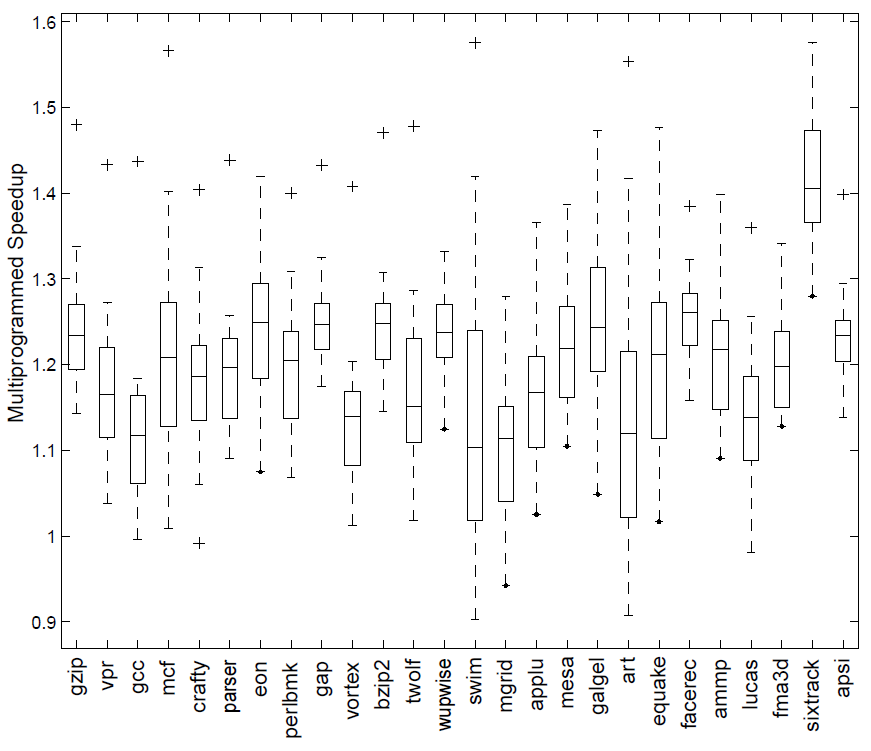
\includegraphics[width=0.9\textwidth]{img/smt.png}
\caption{Speed-up obtinut folosit SMT} \end{figure*}



\section{Concluzii} 
\label{sec:concluzii}
Concluzii ?



\bibliographystyle{abbrv}
\bibliography{roedunet-gateway}

\end{document}
